\newpage

% Definido um novo cabeçalho com o título do elemento atual
\fancypagestyle{tituloanexoapendice}[plain]{
    \fancyhead[C]{\bfseries\uppercase{Apêndice A - Plano da revisão sistemática}}
}

% Resolvendo bug de erro de pagina no hyperref e definindo nova entrada do sumário
\phantomsection
\addcontentsline{toc}{chapter}{\MakeUppercase{Apêndice A - Plano da revisão sistemática}} 

% Inclui apenas a primeira página do PDF, com estilo que tem o titulo desse elemento
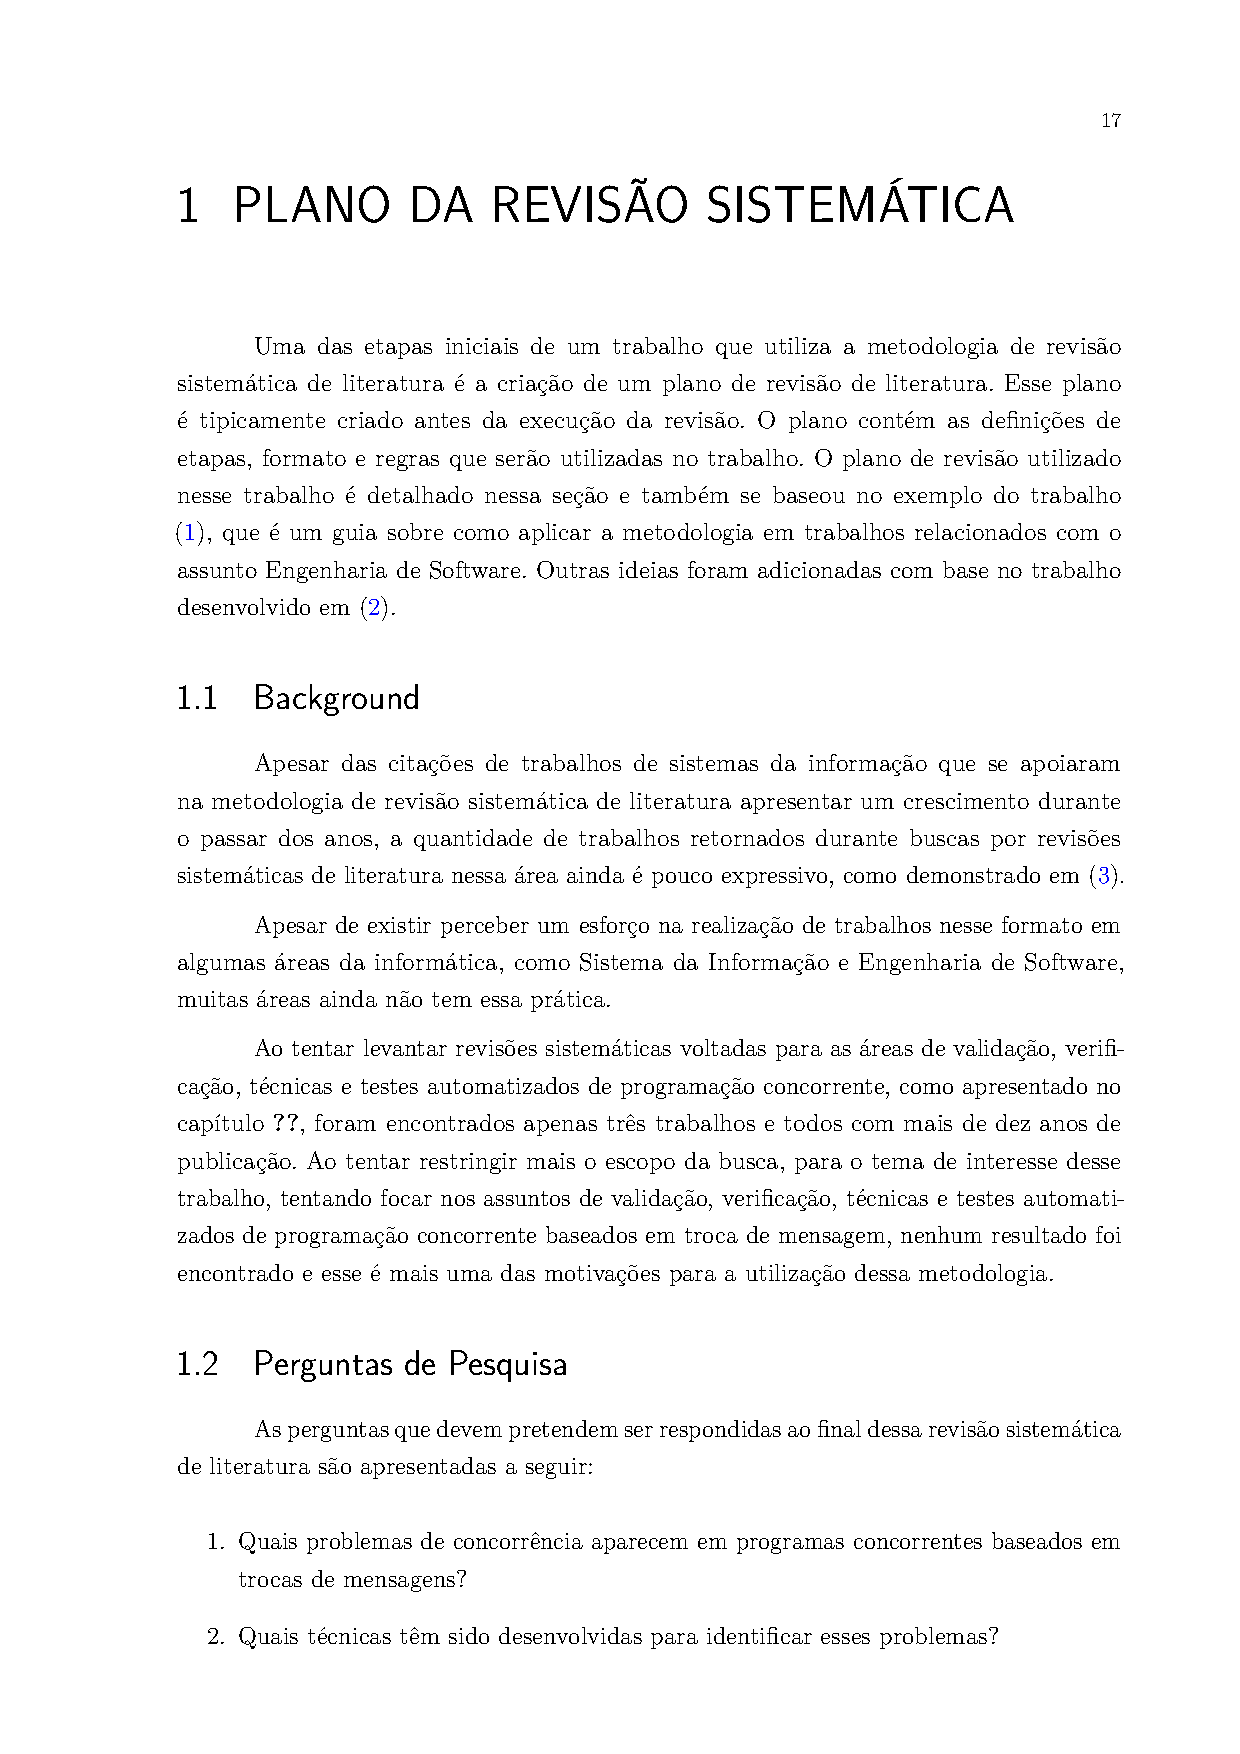
\includepdf[pages=1,scale=0.82,frame=true,pagecommand={\thispagestyle{tituloanexoapendice}}]{metadados/plano_revisao.pdf}

% Inclui da página 2 em diante do PDF, com o cabeçalho padrão apenas com a paginação
\includepdf[pages=2-,scale=0.82,frame=true,pagecommand={\thispagestyle{plain}}]{metadados/plano_revisao.pdf}